\chapter{Evaluation}

In this chapter I will supply enough evidence about how the \ac{MA3C} algorithm learns faster and explores better than
\ac{A3C} in environments where subgoals can be defined.
All the code needed to make the following analysis was developed inside a project of the Universidad Pompeu Fabra researcher
Miquel Juyent.
The \ac{A3C} algorithm was fully provided by him while the algorithm \ac{MA3C} and the games Simple States and Complex
States have been developed by me.
The seed to initialize the weights of the different networks where randomly chosen in each of the experiments and runs.
% TODO PONER EL MONTEZUMA

\section{Simple States}

I have compared the performance of both algorithms \ac{A3C} (\ffref{alg:A3C}) and \ac{MA3C} (\ffref{alg:MA3C}) in Simple
States game (\ffref{subsec:SimpleStates}).

The hyperparameters used for both algorithms are:
\begin{itemize} % TODO PROGUNTAR A MIQUEL QUE FALTA Y SI PONER EL VALUE REGULARIZATION
    \item The discount factor $\gamma = 0.99$.
    \item Batch size $20$. %TODO EXPLAIN
    \item The number of threads in which the algorithms have been parallelized is $8$.
    \item Subtrees $K = 3$. (just for \ac{MA3C})
    \item Entropy regularization term $\beta = 0.1$.
    \item Value regularization term $ = 0.5$ %TODO PONER EN EL ALGORITMO
\end{itemize}

This parameters have been chosen in order to show the disadvantages of \ac{A3C} as opposed to \ac{MA3C}.
There might be a different combination of hyperparameters in which, at the end, both algorithms converge to the same solution.
Since the ultimate goal is to show how \ac{MA3C} explores better, this hyperparameters are good enough.

\begin{figure}[hbtp]
\begin{center}
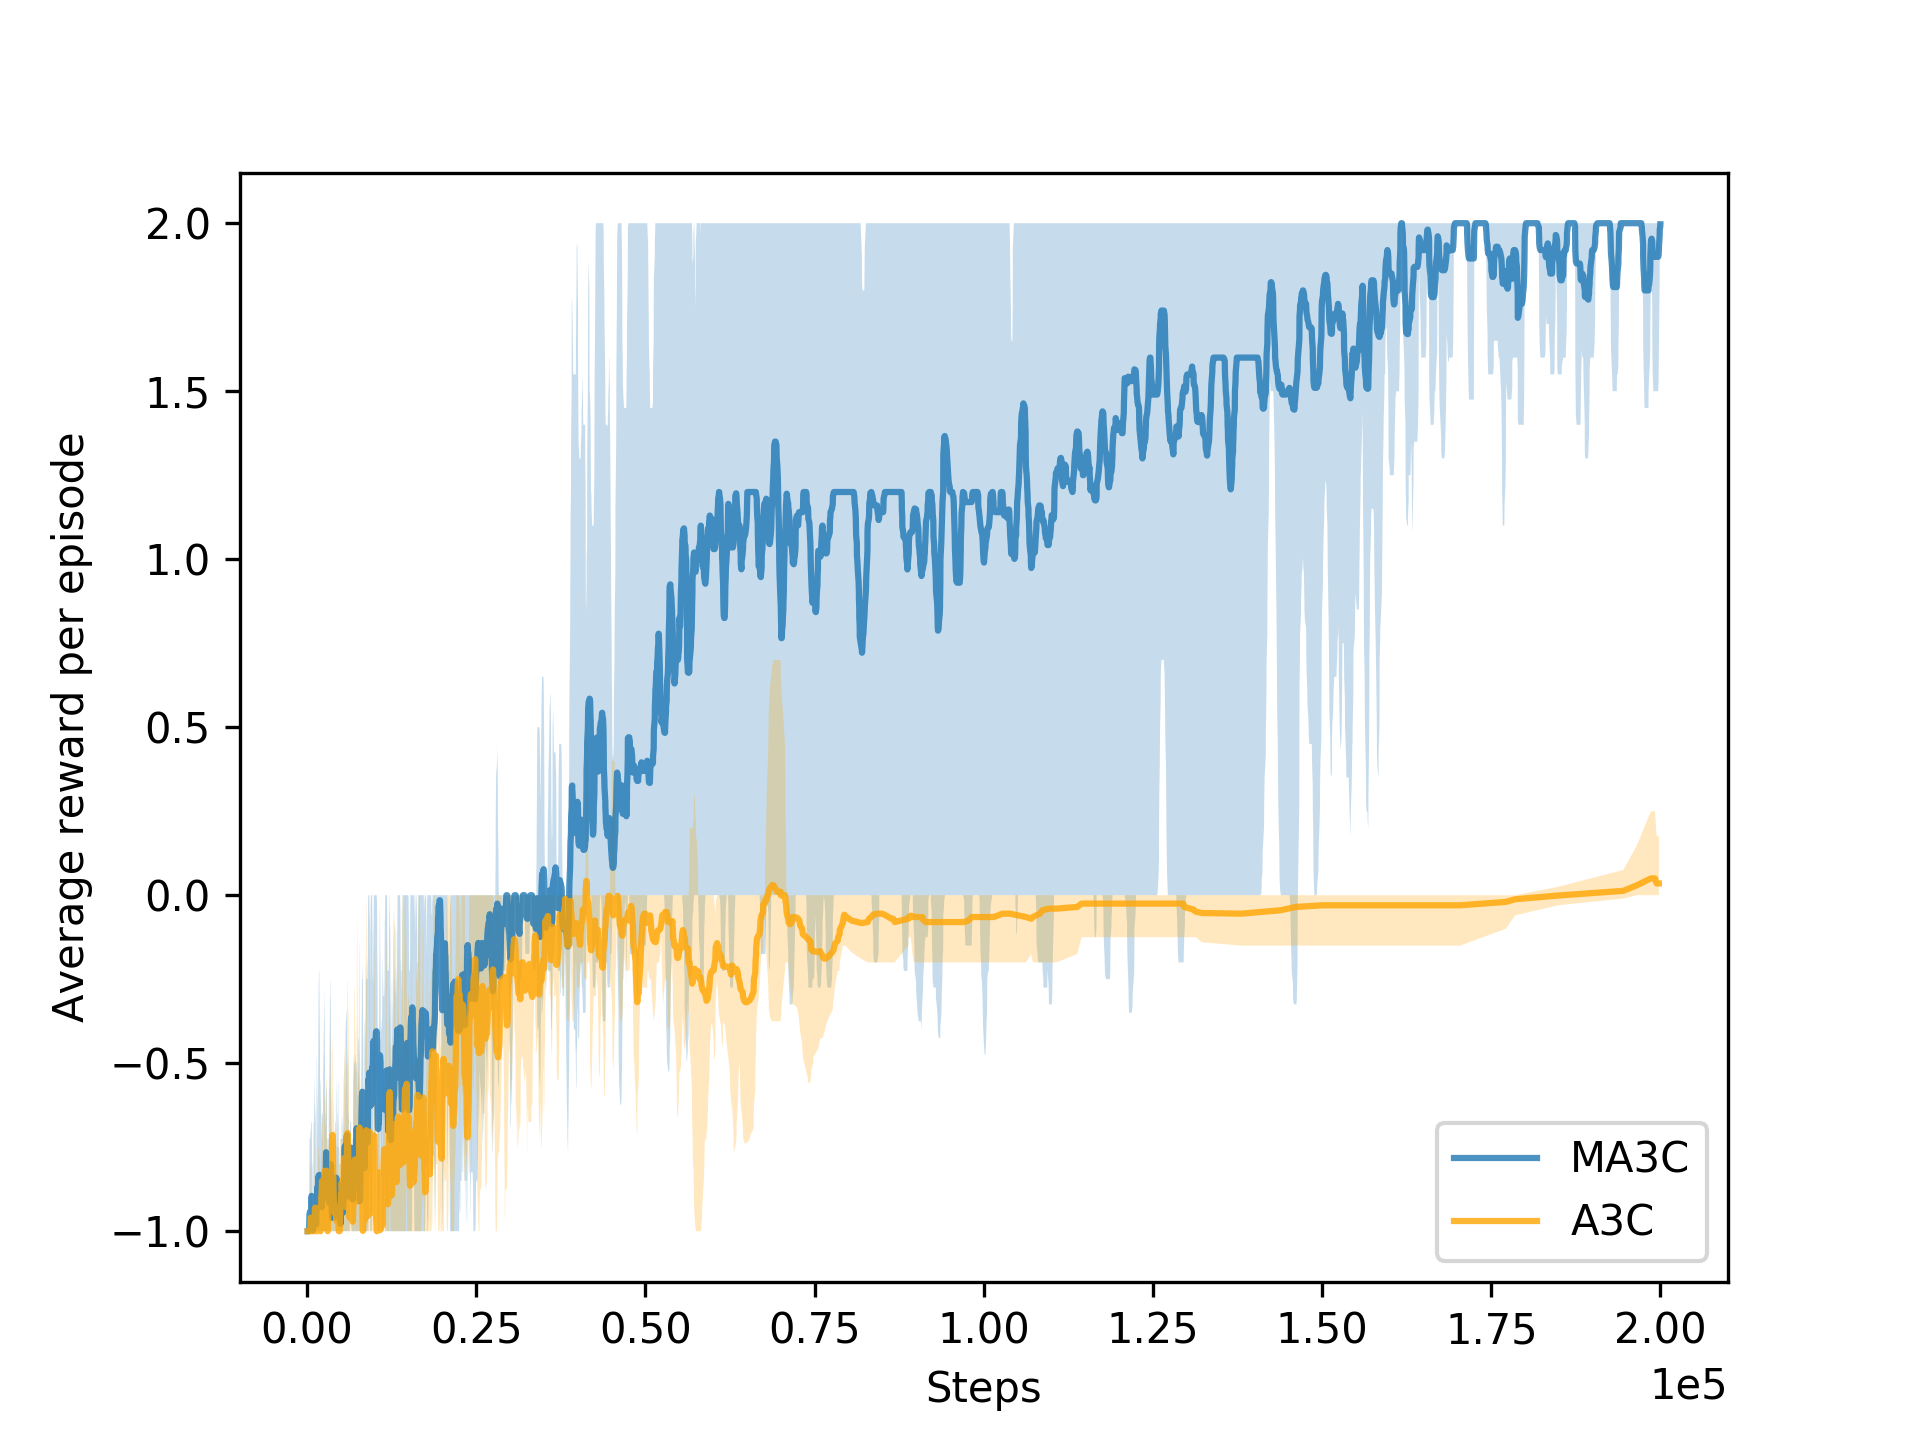
\includegraphics[width=250]{img/SimpleStates_performance.png}
\end{center}
\caption[Simple States performance]
{Average score over $5$ runs of \ac{A3C} and \ac{MA3C} algorithms in Simple States environment (200k steps/actions).
The graphics have been smoothed by a moving average with a $20$ steps window.
The shadow represents maximum and minimum values of those $5$ smoothed runs.}
\label{fig:SimpleStates_performance}
\end{figure}

The learning process of both algorithms measured by score over steps is shown in \ffref{fig:SimpleStates_performance}.
As can be seen, \ac{MA3C} algorithm obtains score $2$ (checkpoint and door) while \ac{A3C} obtains score $0$ because it
reaches the checkpoint but then hits a wall.

This is due to the subtree changes which the algorithm makes every time it goes through any of the checkpoints (normal
and hidden).
Every time the change happens the data in the common network changes in a different manner (the direction of the gradient) %TODO NO HE HABLADO DEL GRADIENTE , QUITAR?
until it converges to common features for all subtrees.
Thanks to that the randomness is implicitly increased every time the change happens until convergence is achieved.
And, as far as more random actions lead to better exploration, this algorithm is using the subgoals (checkpoints) in
order to enhance exploration only when needed, specifically when a new phase is achieved.

It is important to remember that the hidden checkpoint does not give any reward, so in some cases there will be no need
of adding intermediate rewards, just subtree changes.
In general, when solving a problem with \ac{MA3C} it might be no need of doing reward shaping (\ffref{subsec:RewardShaping})
and carefully select the $\mathcal{F}$ function to ensure near-optimal policies.
The subtree changes can be done in any state and the optimal policies will remain the same, it will just enhance exploration
after reaching that states.

\section{Complex States}

Thanks to the results obtained with Simple States game, we realized that \ac{MA3C} may be better than \ac{A3C} learning
different policies from two really similar states.
We decided to test the algorithms in this game (Complex States, \ffref{subsec:ComplexStates}) in order to observe how they
behave in environments in which it is mandatory to retrace its steps.
It is important to mention that in this game there is no hidden checkpoint, so the \ac{MA3C} does not have as much
``advantage" as in Simple States.

% TODO PONER HYPERPARAMETROS DESPUES DE COMPLETAR LOS ANTERIORES

\begin{figure}[hbtp]
\begin{center}
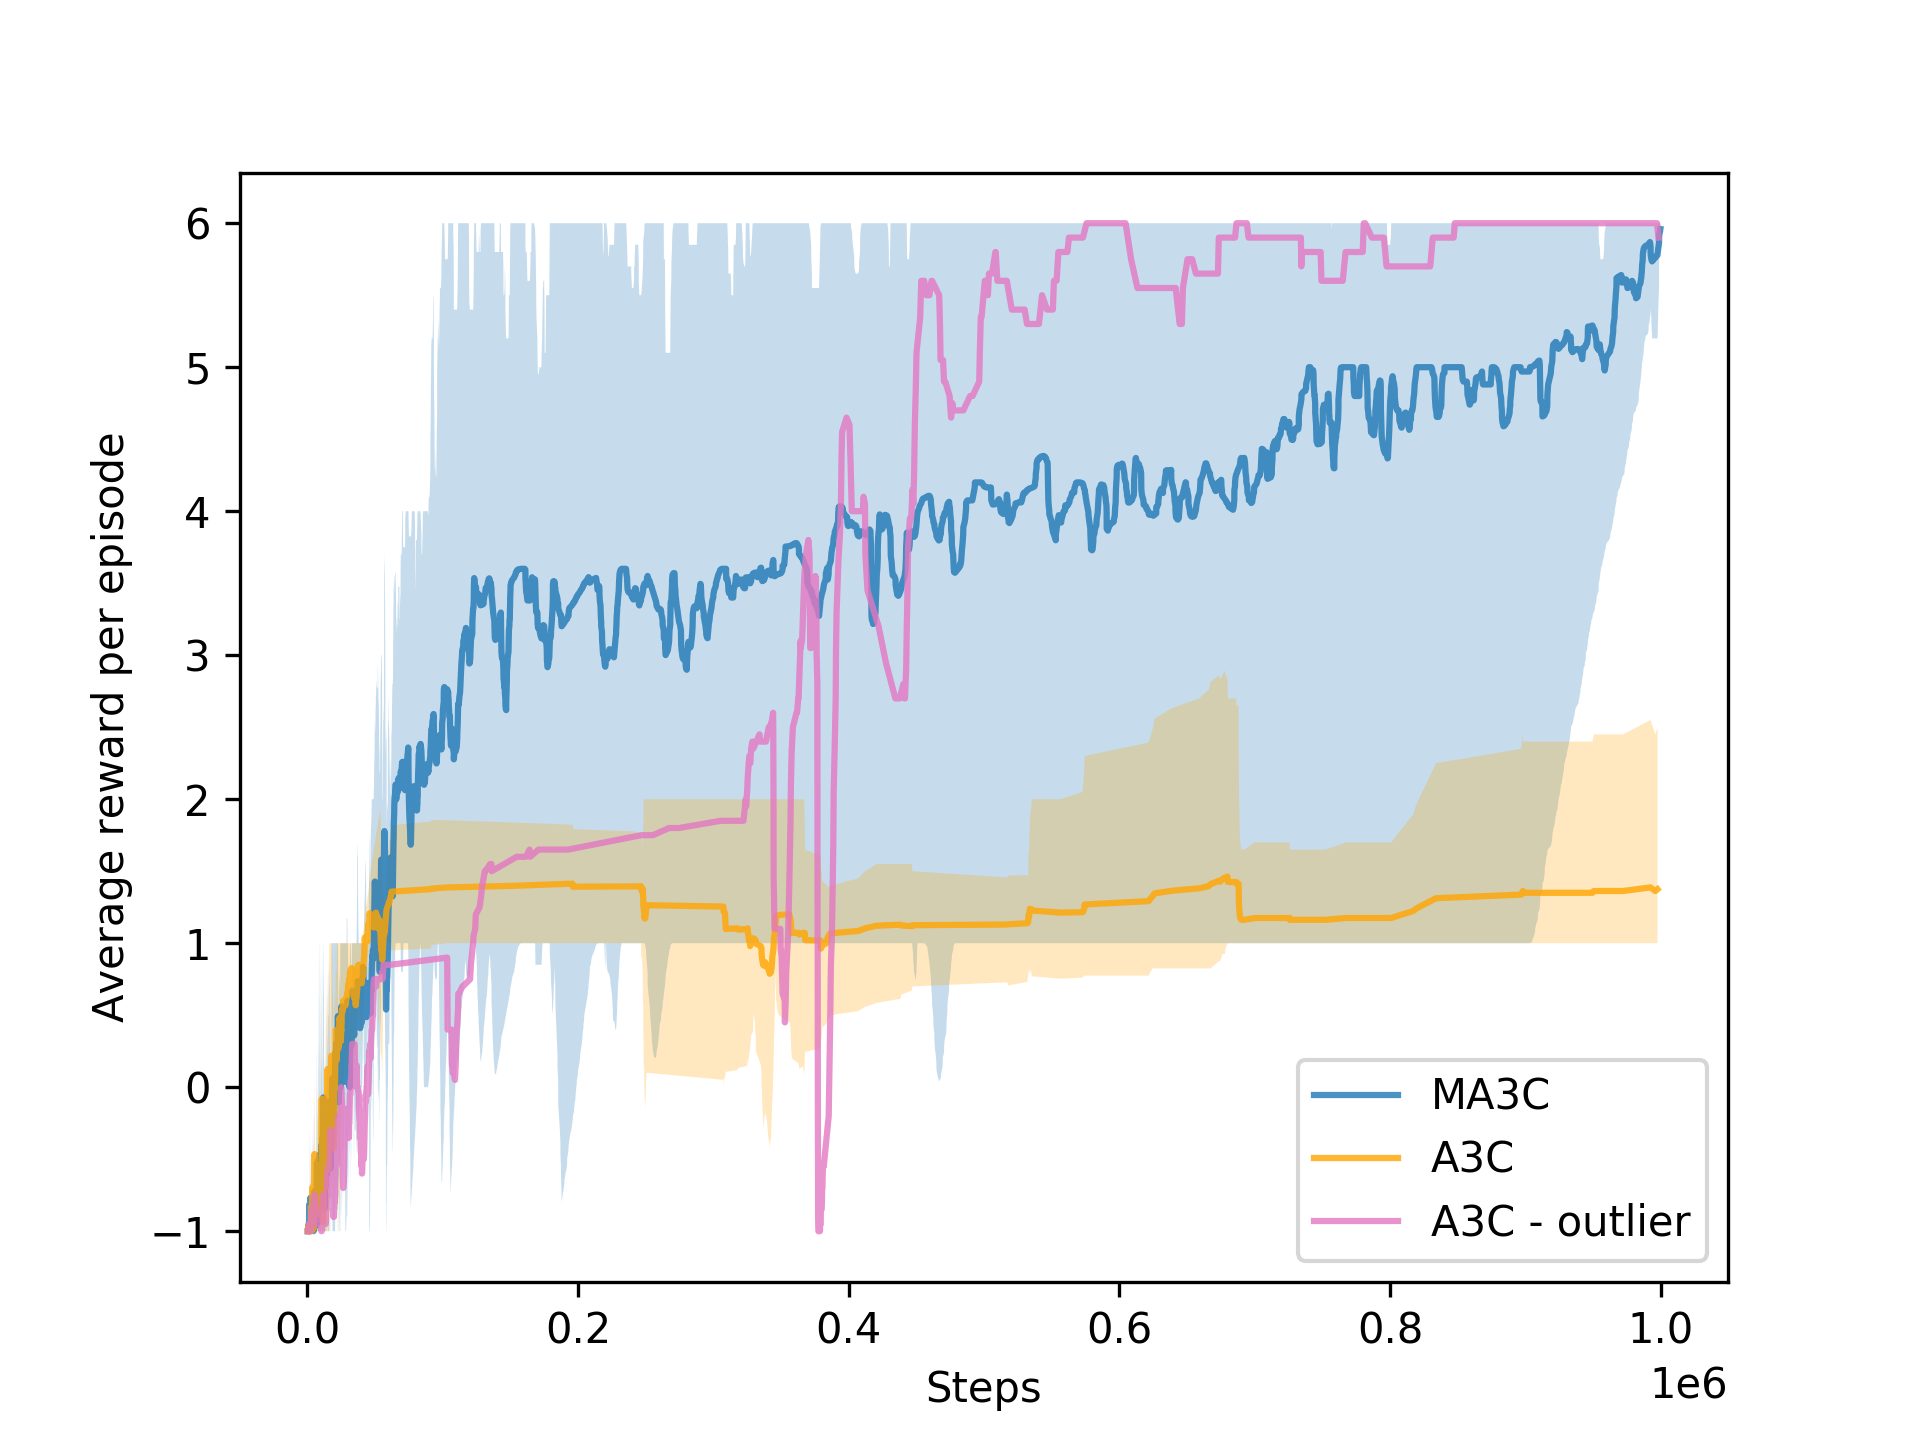
\includegraphics[width=250]{img/ComplexStates_performance.png}
\end{center}
\caption[Complex States performance]
{Average score over $5$ runs of \ac{A3C} and \ac{MA3C} algorithms in Complex States environment (1M steps/actions).
The best run that I obtained with \ac{A3C} is shown as an outlier because it was the only run in which I was able to get
reward $6$.
The graphics have been smoothed by a moving average with a $20$ steps window.
The shadow represents maximum and minimum values of those $5$ smoothed runs.}
\label{fig:ComplexStates_performance}
\end{figure}

The learning process of both algorithms measured by score over steps is shown in \ffref{fig:ComplexStates_performance}.
As can be seen, \ac{MA3C} algorithm obtains score $6$ (all checkpoints and doors) while \ac{A3C} obtains score about $1.5$ on average,
which means that half the time it reaches the first door and the other half it only reaches the second checkpoint
(at the end both times hits the wall).
The outlier drawn as a pink line is low probable case of \ac{A3C} in which it succeeds, obtaining also score $6$.

With this results we can observe how \ac{MA3C} performs better, not only in terms of exploration but also in average succeed.
Going back into his steps may be a difficult task for \ac{A3C} because of the similarity of inputs.
That is, if the policy learned when being next to the first checkpoint is to take the \textsc{UP} action, while coming back
from the second checkpoint to the first one, the policy must change in order to take the \textsc{DOWN} action.
In both cases the hero will be next to the first checkpoint, so the algorithm must figure out that, the location change
of the door, means a change on the goal.

Using \ac{MA3C} in this kind of problems allows us to change the goal of the agent very easily, just by selecting another
subtree.
Since the unique layer which changes is the last one, we will preserve all the previous knowledge about the environment
while learning how to reach the new goal.


\section{Montezuma's Revenge}
% TODO WE OR I BUT NOT BOTH
% TODO PODRÍA HACER UN EXPERIMENTO SIN REWARD SHAPING PERO CAMBIANDO DE SUBTREE A VER QUE SALE

The hyperparameters selected are almost the same than in Simple States and Complex States, the only ones that change are
the following:
\begin{itemize}
    \item The number of threads in which the algorithms have been parallelized is $32$ in order to speed up the learning
    process.
    \item Subtrees $K = 4$, one for each option which the algorithm must learn. (just for \ac{MA3C})
\end{itemize}
% TODO PONER HYPERPARAMETROS DESPUES DE COMPLETAR LOS ANTERIORES, RECORDAR K=?

\begin{figure}[hbtp]
\begin{center}
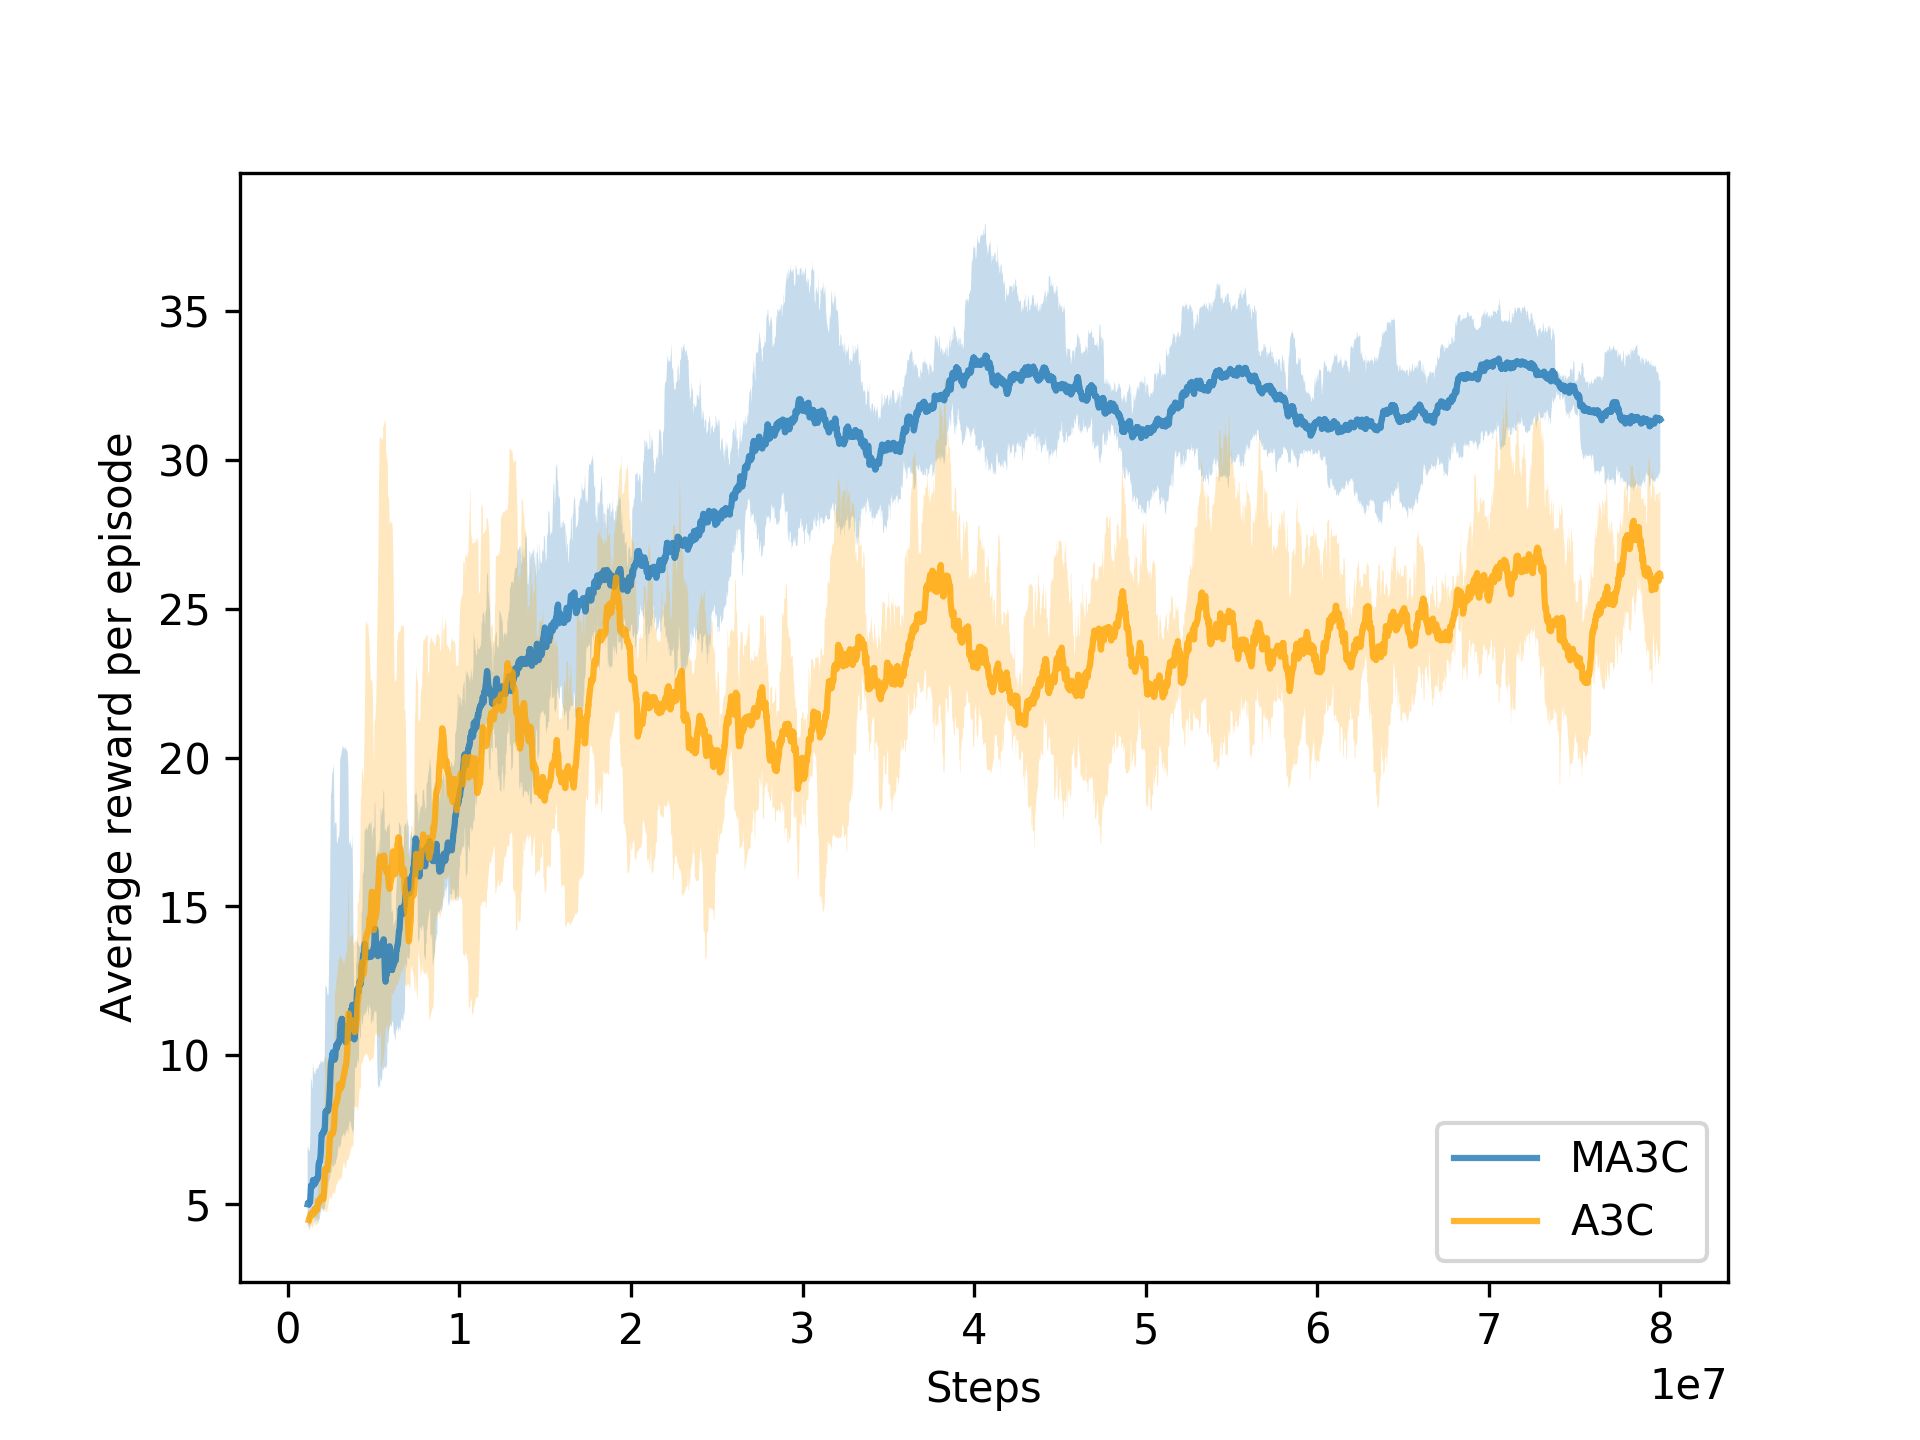
\includegraphics[width=250]{img/Montezuma_performance.png}
\end{center}
\caption[Montezuma's Revenge performance]
{Average score over $5$ runs of \ac{A3C} and \ac{MA3C} algorithms in Simple States environment (80M steps/actions).
The graphics have been smoothed by a moving average with a $20$ steps window.
The shadow represents maximum and minimum values of those $5$ smoothed runs.}
\label{fig:Montezuma_performance}
\end{figure}

As explained in \ffref{subsec:MontezumasRevenge}, the algorithm is learning the different options of the problem (which are
being executed one after the other).
After doing an 80 million steps training, it was able to reach the third checkpoint (Lstairs) in many runs, while reaching
the key in just a few of them.
So it successfully learned the policies of options $o_0$, $o_1$ and $o_2$, and it was trying to learn $o_3$.
This is not fully true because the reward of completing $o_3$ is 110 while the others rewards are just 10, but we can
affirm that with this training process we obtain policies which reach Lstairs with high probability.
As in the other experiments, there might be a different combination of hyperparameters which performs better than in this experiment,
but this ones are good enough to show the differences between both algorithms.

% TODO VER QUE TODAS LAS GRAFICAS SE QUEDEN BIEN
% TODO IT O HE PARA REFERIRSE A LOS ALGORITMOS PERO NO AMBAS.

As can be seen in \ffref{fig:Montezuma_performance}, the learning process of \ac{MA3C} is faster than \ac{A3C}.
Even in complex environments as this one is, the main knowledge can be resumed in the first layers and changing the
subtree is useful to model different subgoals/options.
The \ac{MA3C} curve is also less noisy than \ac{A3C}, which means that this algorithm is less susceptible to
behaviour changes during the learning process.

%%% Local Variables: 
%%% mode: latex
%%% TeX-master: "../report"
%%% End: 